\section{Durchführung}
Für den Versuch wurde ein Aufbau gemäß der Fraunhoferschen Versuchsanordnung verwendet, wie er in der Skizze dargestellt ist.
Das Licht des Lasers wird am Spalt gebeugt, welcher individuell zwischen Einzel- und Doppelspalt gewechselt werden kann.
Die Intensität wird mithilfe eines photosensitiven Elementes gemessen, welches parallel zum Spalt in einem $5cm$ breiten 
Intervall verschoben werden kann. \\
\begin{figure}[h]
    \centering
    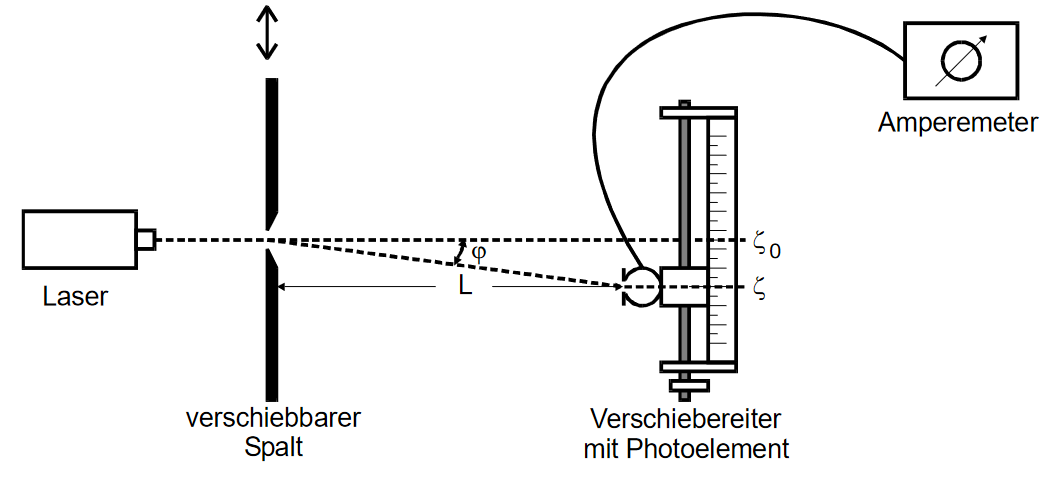
\includegraphics{Beugung am Spalt Versuchsanordnung}
    \caption{Versuchsanordnung}
  \end{figure}
Da das Photelement auch ohne angeschalteten Laser bereits einen Strom anzeigt, muss für akkurate Ergebnisse zunächst 
dieser Dunkelstrom gemessen werden. Anschließend wird für zunächst für den Einzelspalt die Position des Detektors variirt und
der Strom gemessen wird. Anschließend wird eine analoge Messung für den Doppelspalt durchgeführt.
